\subsubsection{Notifications}

\begin{center}
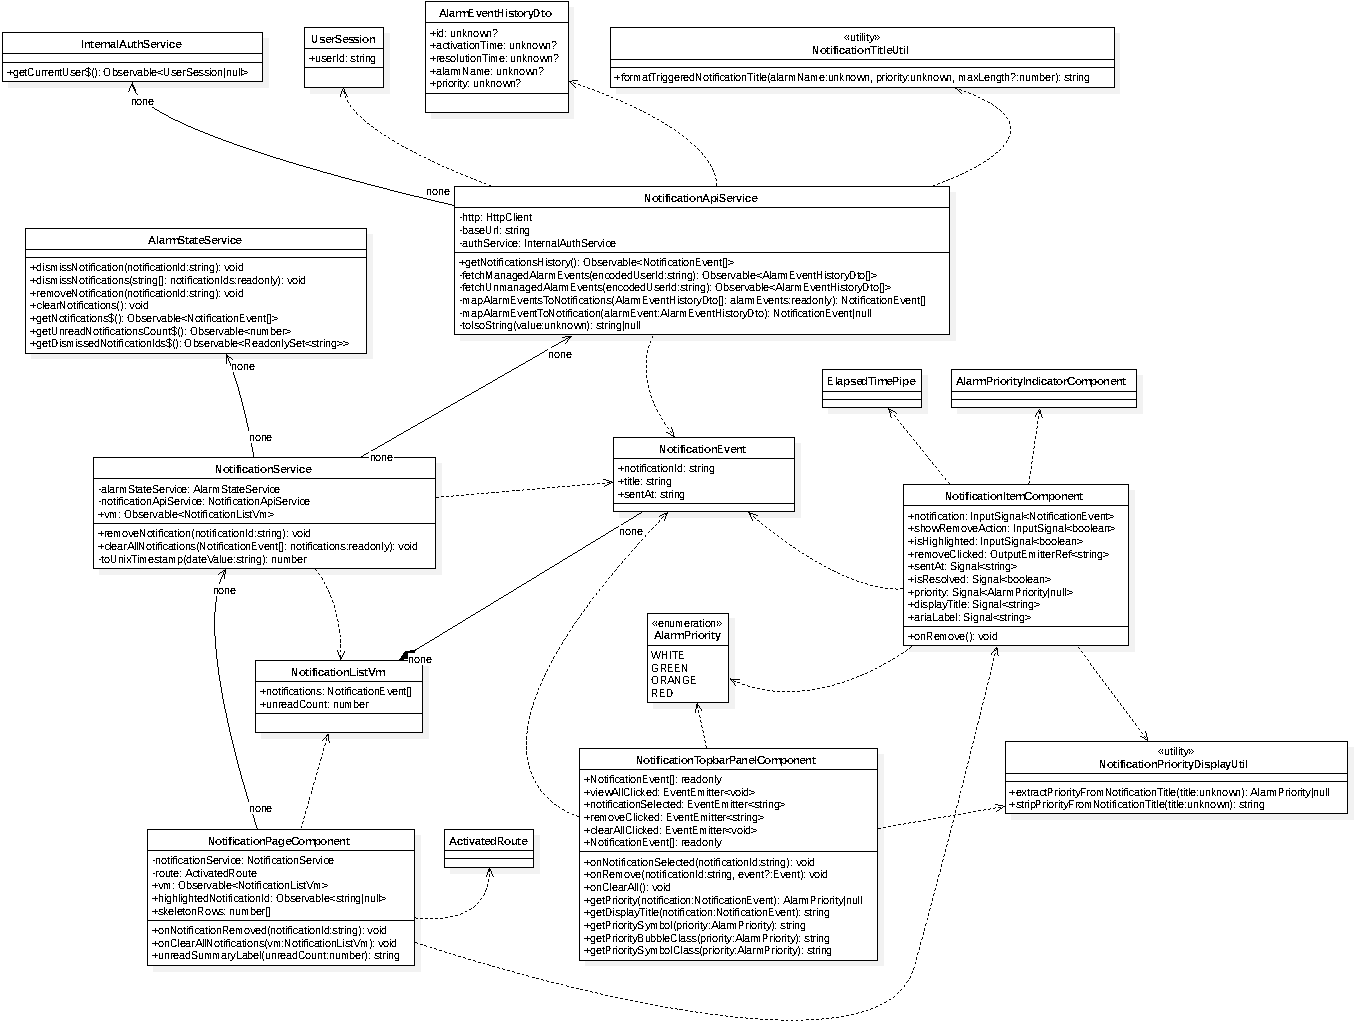
\includegraphics[width=\textwidth]{./frontend/notifications/notification.pdf}
\captionof{figure}{Diagramma delle classi del modulo Notifications}
\end{center}


\addAtr{+}{count: InputSignal$<$number$>$}{}
\addAtr{-}{unreadCount: Signal$<$number$>$}{}
\addAtr{+}{isVisible: Signal$<$boolean$>$}{}
\addAtr{+}{displayCount: Signal$<$string$>$}{}
\addAtr{+}{ariaLabel: Signal$<$string$>$}{}
\makeCl{NotificationBadgeComponent}{Componente Angular che visualizza un badge con il conteggio delle notifiche non lette. Limita il valore visualizzato a 99+ e si nasconde automaticamente quando il conteggio è zero.}

\addAtr{+}{notification: InputSignal$<$NotificationEvent$>$}{}
\addAtr{+}{showRemoveAction: InputSignal$<$boolean$>$}{}
\addAtr{+}{isHighlighted: InputSignal$<$boolean$>$}{}
\addAtr{+}{removeClicked: OutputEmitterRef$<$string$>$}{}
\addAtr{+}{sentAt: Signal$<$Date$>$}{}
\addAtr{+}{isResolved: Signal$<$boolean$>$}{}
\addAtr{+}{priority: Signal$<$AlarmPriority $|$ null$>$}{}
\addAtr{+}{displayTitle: Signal$<$string$>$}{}
\addAtr{+}{ariaLabel: Signal$<$string$>$}{}
\addMet{+}{onRemove() : void}{Emette l'evento removeClicked con l'identificativo della notifica corrente.}
\makeCl{NotificationItemComponent}{Componente Angular che visualizza una singola notifica con priorità, titolo, data e azione di rimozione opzionale. Calcola dinamicamente lo stato di risoluzione e la priorità a partire dal titolo della notifica.}

\addAtr{-}{notificationService: NotificationService}{}
\addAtr{-}{route: ActivatedRoute}{}
\addAtr{+}{vm\$: Observable$<$NotificationListVm$>$}{}
\addAtr{+}{highlightedNotificationId\$: Observable$<$string $|$ null$>$}{}
\addAtr{+}{skeletonRows: number[]}{}
\addMet{+}{onNotificationRemoved(notificationId: string) : void}{Delega al servizio la rimozione della notifica con l'identificativo specificato.}
\addMet{+}{onClearAllNotifications(vm: NotificationListVm) : void}{Delega al servizio la cancellazione di tutte le notifiche presenti nel view model.}
\addMet{+}{unreadSummaryLabel(unreadCount: number) : string}{Restituisce l'etichetta testuale che riassume il numero di notifiche non lette, gestendo il caso singolare e plurale.}
\makeCl{NotificationPageComponent}{Componente Angular che rappresenta la pagina delle notifiche, con supporto alla visualizzazione, rimozione e cancellazione in blocco. Recupera l'identificativo della notifica da evidenziare tramite i parametri di query dell'URL.}

\addAtr{+}{notifications: ReadonlyArray$<$NotificationEvent$>$}{}
\addAtr{+}{viewAllClicked: EventEmitter$<$void$>$}{}
\addAtr{+}{notificationSelected: EventEmitter$<$string$>$}{}
\addAtr{+}{removeClicked: EventEmitter$<$string$>$}{}
\addAtr{+}{clearAllClicked: EventEmitter$<$void$>$}{}
\addAtr{-}{maxVisibleNotifications: number}{}
\addMet{+}{visibleNotifications() : ReadonlyArray$<$NotificationEvent$>$}{Restituisce le prime notifiche fino al limite massimo di visibilità configurato.}
\addMet{+}{onNotificationSelected(notificationId: string) : void}{Emette l'evento notificationSelected con l'identificativo della notifica selezionata.}
\addMet{+}{onRemove(notificationId: string, event?: Event) : void}{Emette l'evento removeClicked con l'identificativo della notifica, interrompendo la propagazione dell'evento DOM se fornito.}
\addMet{+}{onClearAll() : void}{Emette l'evento clearAllClicked per richiedere la cancellazione di tutte le notifiche.}
\addMet{+}{getPriority(notification: NotificationEvent) : AlarmPriority $|$ null}{Estrae la priorità dalla notifica a partire dal titolo tramite la funzione di utilità dedicata.}
\addMet{+}{getDisplayTitle(notification: NotificationEvent) : string}{Restituisce il titolo della notifica privo del prefisso di priorità, usando il titolo originale come fallback.}
\addMet{+}{getPrioritySymbol(priority: AlarmPriority) : string}{Restituisce il simbolo testuale associato al livello di priorità specificato.}
\addMet{+}{getPriorityBubbleClass(priority: AlarmPriority) : string}{Restituisce le classi CSS per il bubble di priorità in base al livello specificato.}
\addMet{+}{getPrioritySymbolClass(priority: AlarmPriority) : string}{Restituisce le classi CSS per il simbolo di priorità in base al livello specificato.}
\makeCl{NotificationTopbarPanelComponent}{Componente Angular che visualizza un pannello compatto delle notifiche nella topbar, limitando la lista alle prime notifiche visibili. Espone eventi per la selezione, rimozione e cancellazione delle notifiche e gestisce la presentazione visiva delle priorità.}

\addAtr{+}{notificationId: string}{}
\addAtr{+}{title: string}{}
\addAtr{+}{sentAt: string}{}
\addAtr{+}{eventType?: 'triggered' $|$ 'resolved'}{}
\makeAbCl{NotificationEvent}{Interfaccia che rappresenta una singola notifica di sistema, condivisa tra lo storico HTTP e gli eventi push real-time. La simmetria tra le due sorgenti consente a NotificationService di unirle senza trasformazioni intermedie.}

\addAtr{+}{notifications: NotificationEvent[]}{}
\addAtr{+}{unreadCount: number}{}
\makeAbCl{NotificationListVm}{Interfaccia che rappresenta il view model della pagina delle notifiche, prodotto da NotificationService tramite combineLatest. Aggrega la lista unificata e deduplicata delle notifiche e il contatore delle non lette in un unico snapshot atomicamente coerente.}

\addAtr{-}{alarmStateService: AlarmStateService}{}
\addAtr{-}{notificationApiService: NotificationApiService}{}
\addAtr{+}{vm\$: Observable$<$NotificationListVm$>$}{}
\addMet{+}{removeNotification(notificationId: string) : void}{Rimuove la notifica specificata dallo stato locale e la marca come letta tramite il servizio di stato degli allarmi.}
\addMet{+}{clearAllNotifications(notifications: ReadonlyArray$<$NotificationEvent$>$) : void}{Marca come lette e rimuove tutte le notifiche fornite dallo stato locale.}
\addMet{-}{toUnixTimestamp(dateValue: string) : number}{Converte una stringa data in timestamp Unix, restituendo zero se il valore non è parsabile.}
\makeCl{NotificationService}{Servizio Angular con scope a livello di componente che compone le notifiche storiche HTTP e quelle in-session push in un unico view model reattivo. Gestisce la deduplicazione, il filtraggio delle notifiche dismesse e l'ordinamento per data decrescente.}

\addAtr{-}{http: HttpClient}{}
\addAtr{-}{baseUrl: string}{}
\addAtr{-}{authService: InternalAuthService}{}
\addAtr{-}{HISTORY\_LIMIT: number}{}
\addAtr{-}{HISTORY\_OFFSET: number}{}
\addMet{+}{getNotificationsHistory() : Observable$<$NotificationEvent[]$>$}{Recupera la cronologia completa delle notifiche per l'utente corrente combinando gli eventi di allarme gestiti e non gestiti.}
\addMet{-}{fetchManagedAlarmEvents(encodedUserId: string) : \\ Observable$<$AlarmEventHistoryDto[]$>$}{Esegue una chiamata API per recuperare gli eventi di allarme che sono già stati presi in carico o risolti.}
\addMet{-}{fetchUnmanagedAlarmEvents(encodedUserId: string) : \\ Observable$<$AlarmEventHistoryDto[]$>$}{Effettua una richiesta HTTP per ottenere l'elenco degli eventi di allarme ancora attivi o non gestiti.}
\addMet{-}{mapAlarmEventsToNotifications(alarmEvents: ReadonlyArray$<$AlarmEventHistoryDto$>$) : NotificationEvent[]}{Trasforma un insieme di oggetti DTO provenienti dal backend in una lista di eventi di notifica pronti per l'interfaccia.}
\addMet{-}{mapAlarmEventToNotification(alarmEvent: AlarmEventHistoryDto) : NotificationEvent $|$ null}{Converte un singolo evento di allarme nel formato standard di notifica, determinando il titolo e il timestamp corretti.}
\addMet{-}{toIsoString(value: unknown) : string $|$ null}{Normalizza diversi formati di data in una stringa conforme allo standard ISO per garantire la coerenza temporale.}
\makeCl{NotificationApiService}{Questo servizio centralizza il recupero della cronologia delle notifiche tramite API REST, integrando i dati provenienti dal sistema di gestione allarmi. Si occupa della mappatura dei dati grezzi in modelli di notifica fruibili dai componenti UI.}